\documentclass[12pt]{report}

% greek hyphenation package
\usepackage{fontspec}
\usepackage{xgreek}
\usepackage{amsmath}
\usepackage{amsfonts}
\usepackage{amssymb}
\usepackage{bm}

\newcommand{\norm}[1]{\left\lVert #1 \right\rVert_2}
\newcommand{\abs}[1]{\left\vert #1 \right\vert}

\usepackage{fancyhdr}
\usepackage{sectsty}

\usepackage{array}
\usepackage{multirow}
%~ \usepackage{adjustbox}
\usepackage{hyperref}
\hypersetup{
    colorlinks=true,
    linkcolor=blue,
    filecolor=magenta,
    urlcolor=cyan,
}



\usepackage{float}
\usepackage{framed}
\restylefloat{table}

\usepackage[utf8]{inputenc}
\usepackage{algorithm,algorithmicx,algpseudocode}

\algnewcommand{\LineComment}[1]{\State \# #1}
\renewcommand{\algorithmicrequire}{\textbf{Input:}}
\renewcommand{\algorithmicensure}{\textbf{Output:}}


\DeclareTextFontCommand\emphcolor{\bfseries\color{blue}}

\usepackage[margin=1in,footskip=0.40in]{geometry}

\usepackage{listings}
\usepackage{xcolor}

\usepackage{graphicx}
\usepackage[justification=centering,labelfont=bf]{caption}
\usepackage{subcaption}
\graphicspath{{images/}}

\usepackage{datetime}
\usepackage{polyglossia}
\setmainlanguage{greek}

\setlength{\parindent}{4em}
\setlength{\parskip}{1em}

\usepackage[normalem]{ulem}
\usepackage[uppercase]{titlesec}

\allsectionsfont{\centering}
\titleformat{\chapter}
{\Huge\bfseries\filcenter}{\uline{\thechapter.\ }}{0em}{\uline}
\titleformat{\section}
{\Large\bfseries\filcenter}{\uline{\thesection.\ }}{0em}{\uline}
\titleformat{\subsection}{\large\filcenter}{\uline{\thesubsection.\ }}{0em}{\uline}
\titleformat{\subsubsection}{\normalsize\filright}{\uline{\thesubsubsection.}}{0em}{\uline}
\setmainfont[Mapping=tex-text]{DejaVu Sans}
\newfontfamily\greekfont[Script=Greek]{DejaVu Sans}

\usepackage{listings}
\usepackage{xcolor}

\definecolor{mygreen}{rgb}{0,0.6,0}
\definecolor{mygray}{rgb}{0.5,0.5,0.5}
\definecolor{mymauve}{rgb}{0.58,0,0.82}

\lstset{literate=
  {á}{{\'a}}1 {é}{{\'e}}1 {í}{{\'i}}1 {ó}{{\'o}}1 {ú}{{\'u}}1
  {Á}{{\'A}}1 {É}{{\'E}}1 {Í}{{\'I}}1 {Ó}{{\'O}}1 {Ú}{{\'U}}1
  {à}{{\`a}}1 {è}{{\`e}}1 {ì}{{\`i}}1 {ò}{{\`o}}1 {ù}{{\`u}}1
  {À}{{\`A}}1 {È}{{\'E}}1 {Ì}{{\`I}}1 {Ò}{{\`O}}1 {Ù}{{\`U}}1
  {ä}{{\"a}}1 {ë}{{\"e}}1 {ï}{{\"i}}1 {ö}{{\"o}}1 {ü}{{\"u}}1
  {Ä}{{\"A}}1 {Ë}{{\"E}}1 {Ï}{{\"I}}1 {Ö}{{\"O}}1 {Ü}{{\"U}}1
  {â}{{\^a}}1 {ê}{{\^e}}1 {î}{{\^i}}1 {ô}{{\^o}}1 {û}{{\^u}}1
  {Â}{{\^A}}1 {Ê}{{\^E}}1 {Î}{{\^I}}1 {Ô}{{\^O}}1 {Û}{{\^U}}1
  {œ}{{\oe}}1 {Œ}{{\OE}}1 {æ}{{\ae}}1 {Æ}{{\AE}}1 {ß}{{\ss}}1
  {ű}{{\H{u}}}1 {Ű}{{\H{U}}}1 {ő}{{\H{o}}}1 {Ő}{{\H{O}}}1
  {ç}{{\c c}}1 {Ç}{{\c C}}1 {ø}{{\o}}1 {å}{{\r a}}1 {Å}{{\r A}}1
  {€}{{\EUR}}1 {£}{{\pounds}}1
}

\lstdefinestyle{MyMatlab}{%
  backgroundcolor=\color{white},   % choose the background color; you must add \usepackage{color} or \usepackage{xcolor}
  breakatwhitespace=false,         % sets if automatic breaks should only happen at whitespace
  breaklines=true,                 % sets automatic line breaking
  captionpos=b,                    % sets the caption-position to bottom
  frame=single,	                   % adds a frame around the code
  keepspaces=true,                 % keeps spaces in text, useful for keeping indentation of code (possibly needs columns=flexible)
  language=Matlab,                 % the language of the code
  numbers=left,                    % where to put the line-numbers; possible values are (none, left, right)
  numbersep=5pt,                   % how far the line-numbers are from the code
  rulecolor=\color{black},         % if not set, the frame-color may be changed on line-breaks within not-black text (e.g. comments (green here))
  stepnumber=1,                    % the step between two line-numbers. If it's 1, each line will be numbered
  tabsize=2,	                   % sets default tabsize to 2 spaces
  numberstyle=\tiny\color{black}, % the style that is used for the line-numbers
  keywordstyle=\bfseries\color{black},
  commentstyle=\itshape\color{mygray},
  identifierstyle=\color{blue},
}

\pagestyle{fancy}
\fancyhf{}

\fancyhead[R]{\today}
\fancyhead[L]{\thechapter}
\fancyfoot[C]{\thepage}
\renewcommand{\footrulewidth}{1.5pt}% Default \footrulewidth is 0pt
\renewcommand{\headrulewidth}{2pt}

\newcommand{\sectionformat}{\centering}

\begin{document}

% \setcounter{secnumdepth}{3}
\setcounter{tocdepth}{3}

\begin{titlepage}
    \begin{center}
        \vspace*{1cm}

        \Large
        \textbf{Συστήματα Πολυμέσων \& Εικονική Πραγματικότητα}\\

        \large 9\textsuperscript{ο} Εξάμηνο


        \vspace*{0.5cm}

        \Huge
        \uline{Εργασία 2015-2016}\\

        \vspace{1.5cm}

        \large
        \textbf{Παπουδάκης Γεώργιος 7753 papoudak@auth.gr\\
          Χούτας Βασίλειος 7800 vasilis4ch@gmail.com}\\

        \vfill

        \vspace{0.8cm}

        
\includegraphics[width=0.4\textwidth]{university}

        \vspace{0.8cm}

        \smallskip
        Τμήμα Ηλεκτρολόγων Μηχανικών και Μηχανικών Υπολογιστών\\
        \smallskip1
        Πολυτεχνική Σχολή
        \smallskip
        \\Αριστοτέλειο Πανεπιστήμιο Θεσσαλονίκης\\
        \today

    \end{center}
\end{titlepage}

\thispagestyle{empty}
\newpage

\tableofcontents
\listoftables
\listoffigures
\newpage

\chapter{Επιμέρους συστήματα Κωδικοποιητή και Αποκωδικοποιητή}

\section{Σύστημα Υποδειγματοληψίας}

\par Το πρώτο κομμάτι της κωδικοποίησης είναι η υποδειγματοληψία του αρχικού σήματος. 
Έστω ότι το σήμα που μας δίνετε έχει προκύψει από δειγματοληψία ενός αναλογικού 
σήματος με συχνότητα δειγματοληψίας $f_{s1}$. Αρχικός στόχος του κωδικοποιητή 
είναι η μείωση της συχνότητας δειγματοληψίας στη $f_{s2}$, ώστε να μειωθούν τα δείγματα τα 
οποία χρησιμοποιούμε για να αναπαραστήσουμε το σήμα. Στην περίπτωση της αποκωδικοποίησης 
γίνεται υπερδειγματοληψία ώστε αυτό που θα προκύψει να έχει το ίδιο πλήθος δειγμάτων 
με το αρχικό σήμα. Κάνοντας αλλαγή στη συχνότητα δειγματοληψίας από την $f_{s1}$ στην 
$f_{s2}$ το νέο σήμα που προκύπτει έχει μήκος $floor(\frac{f_{s2}}{f_{s1}}\times
(length(x)-1))$.

\par Η συνάρτηση που υλοποιεί αυτή την διαδικασία είναι η $y=changefs(x,f_{s1},\\f_{s2},
interpMethod)$, $f_{s1}$ η αρχική συχνότητα δειγματοληψίας και $f_{s2}$ η τελική και interpMethod είναι η μέθοδος 
με την οποία προκύπτουν τα δείγματα του y με τη μέθοδο της παρεμβολής. Το τέταρτο αυτό 
όρισμα δεν ζητείται από την εκφώνηση αλλά χρησιμοποιείται σε παρακάτω ερωτήματα. 
Στη συνάρτηση changefs ορίζουμε δύο μεταβλητές. Η πρώτη αντιστοιχεί στα δείγματα του αρχικού σήματος 
x, δηλαδή οριζεται ως πίνακας που έχει στοιχεία μέσα από το 1 έως το μήκος του x, 
ενώ η δεύτερη αντιπροσωπεύει τα δείγματα του y και δημιουργείται από το 1 έως το μήκος 
του x με βήμα $\frac{f_{s1}}{f_{s2}}$, έως το μήκος του x. Τα δύο αυτά διανύσματα 
δίνονται σαν είσοδο στην interp1 του Matlab και μας παράγουν το τελικό y, από το οποίο 
κρατάμε μόνο τα $floor(\frac{f_{s2}}{f_{s1}}\times(length(x)-1))$ πρώτα στοιχεία.

\par Στη συνέχεια για να ελένξουμε την ορθότητα της υλοποίησης μας τρέχουμε την 
συνάρτηση testQ1. Παρακάτω παρουσιάζονται τα διαγράμματα που προκύπτουν.

\begin{figure}
    \centering
\begin{subfigure}[h]{0.49\textwidth}
  \centering
  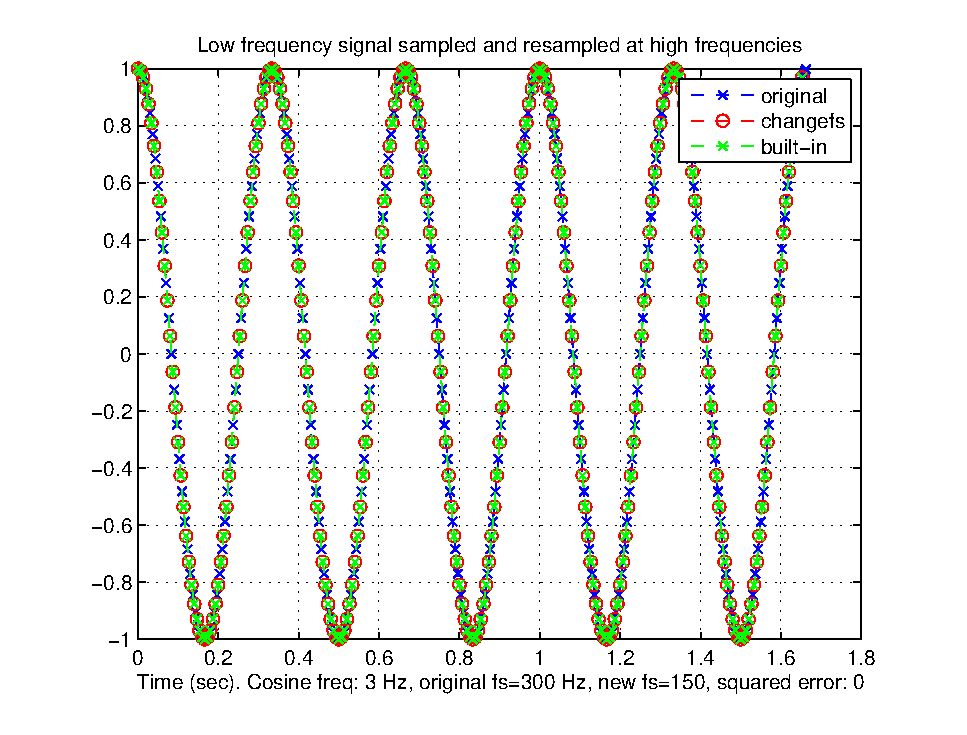
\includegraphics[width=0.4\paperwidth]{test11.eps}
\end{subfigure}
%~ \hfill
\begin{subfigure}[h]{0.49\textwidth}\centering
  \centering
  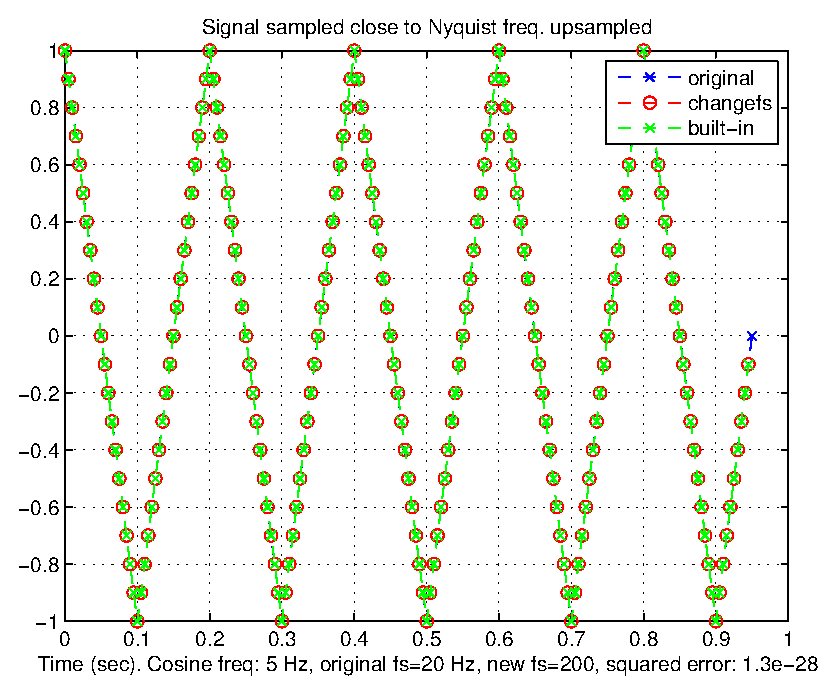
\includegraphics[width=0.4\paperwidth]{test12.eps}
  \end{subfigure}
  %~ \hfill
\begin{subfigure}[h]{0.49\textwidth}
  \centering
  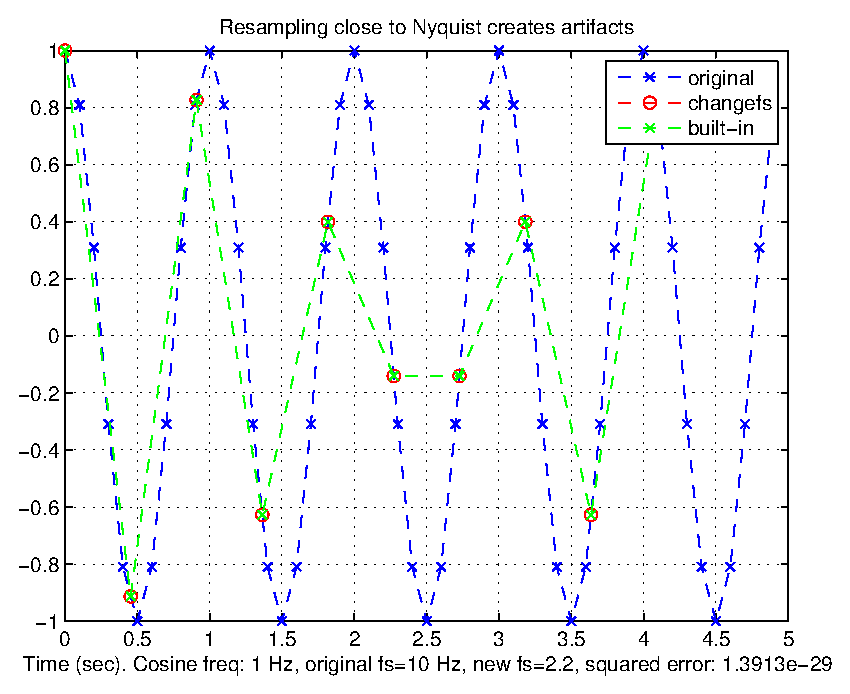
\includegraphics[width=0.4\paperwidth]{test13.eps}
\end{subfigure}
%~ \hfill
\begin{subfigure}[h]{0.49\textwidth}\centering
  \centering
  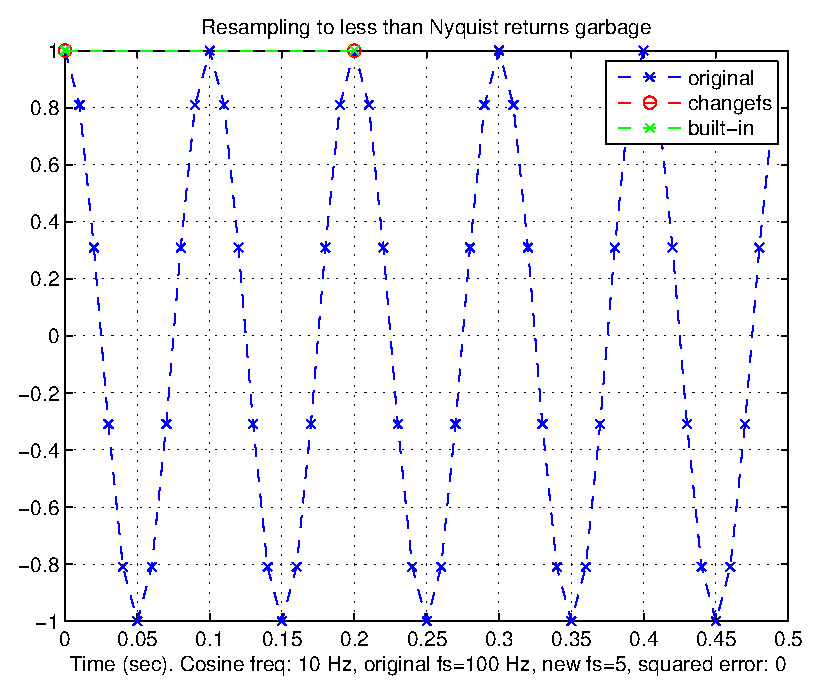
\includegraphics[width=0.4\paperwidth]{test14.eps}
  \end{subfigure}
  %~ \hfill
\end{figure}

\par Παρατηρούμε πως τα σημεία των καμπυλών built-in και changefs ταυτίζονται, 
άρα η υλοποίησή μας είναι σωστή.

\section{Σύστημα Γραμμικής Πρόβλεψης}

\section{Σύστημα Κβαντιστή \& Αποκβαντιστή}

\section{Κωδικοποίηση \& Αποκωδικοποίηση A-DPCM}

\section{Κωδικοποίηση \& Αποκωδικοποίηση Huffman}



\noindent
\begin{minipage}{\linewidth}
\par Το επόμενο βήμα για την υλοποίηση του συστήματος Κωδικοποιητή και Αποκωδικοποιητή που θέλουμε να
αναπτύξουμε είναι η κωδικοποίηση των συμβόλων που αποτελούν το σήμα μας και για αυτό το σκοπό
στρεφόμαστε στην χρήση του κώδικα Huffman.

  \par Ο αλγόριθμος του Huffman βασίζεται στις πιθανότητες εμφάνισης των συμβόλων που μας ενδιαφέρουν
  προκειμένου να εξάγει τον κώδικα που θα χρησιμοποιήσουμε για συμπίεση. Συγκεκριμένα, όσο πιο πιθανό
  είναι ένα σύμβολο, τόσο μικρότερη είναι η συμβολοσειρά που το αναπαριστά. Πρακτικά, μπορεί να
  αναπαρασταθεί από ένα δυαδικό δέντρο, όπου τα φύλλα αντιστοιχούν στα σύμβολα. Για την κατασκευή του
  δέντρου, ξεκινάμε από δύο στοιχεία που έχουν τη μικρότερη πιθανότητα, τα οποία κι ενώνουμε για να
  σχηματίσουμε έναν κόμβο του δέντρο, ο οποίος με την σειρά του θεωρείται ως ένα νέο σύμβολο, με
  πιθανότητα ίση με το άθροισμα των πιθανοτήτων των παιδιών. Στην συνέχεια, επιλέγουμε τα στοιχεία που
  έχουν τις δύο μικρότερες πιθανότητες κι επαναλαμβάνουν την παραπάνω διαδικασία. Ο αλγόριθμος
  τερματίζει όταν όλοι οι κόμβοι έχουν ενωθεί.
  \begin{framed}
    \begin{figure}[H]
      \label{fig:huffman}
      \centering
      \begin{subfigure}{1.0\textwidth}
        \centering
        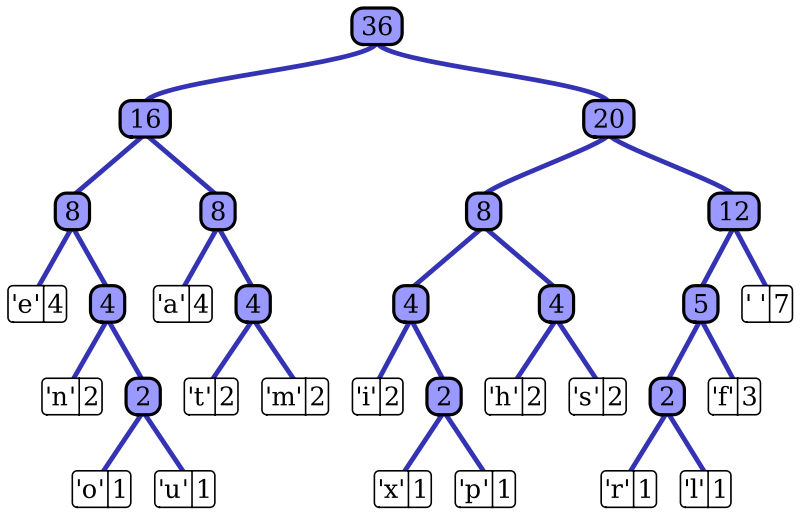
\includegraphics[width=0.8\textwidth]{huffman}
        \caption{\protect{Πηγή: \href{https://en.wikipedia.org/wiki/Huffman\_coding}{Huffman Wikipedia Article}}}
      \end{subfigure}
      \caption{Παράδειγμα Δέντρου Huffman}
    \end{figure}
  \end{framed}
\end{minipage}

\par Η συνάρτηση που κατασκευάζει το παραπάνω δέντρο και κατά συνέπεια και το λεξικό/σύνολο λέξεων
που μας δίνει τον κώδικα Huffman είναι η:
\begin{lstlisting}[style=myMatlab]
  function [s] = huffLUT(p, debug)
\end{lstlisting}
\noindent η οποία αρχικά δημιουργεί μία ουρά προτεραιότητας με κόμβους, όπου κάθε κόμβος είναι ένα
φύλλο που περιέχει ένα από τα αρχικά σύμβολα. Έπειτα, και για όσο υπάρχουν στοιχεία στην ουρά,
εξάγουμε τα δύο στοιχεία με τις χαμηλότερες πιθανότητες, τα ενώνουμε δημιουργώντας έναν νέο κόμβο,
όπως περιγράψαμε παραπάνω και τον οποίο εισάγουμε στην ουρά, αναθέτοντας του και το αντίστοιχο
ψηφίο. Για να εξάγουμε τον κώδικα που αντιστοιχεί σε κάθε σύμβολο, απλά ξεκινάμε από το αντίστοιχο
φύλλο κι ανεβαίνουμε μέχρι την ρίζα του δέντρου, κρατώντας τα ψηφία των κόμβων από τους οποίους
περνάμε.

\par Η συνάρτηση:
\begin{lstlisting}[style=myMatlab]
  function [b] = huff(q, s)
\end{lstlisting}
\noindent κωδικοποιεί την συμβολοσειρά που μας δίνεται με βάση το λεξιλόγιο που δημιούργησε η
\emphcolor{huffLut} αντιστοιχώντας κάθε σύμβολο στον κώδικα του.

\par Τέλος, η συνάρτηση:
\begin{lstlisting}[style=myMatlab]
  function [q, n] = ihuff(b, s, debug)
\end{lstlisting}
\noindent εκτελεί τον αντίστροφο μετασχηματισμό Huffman δοθέντος του λεξιλογίου και μίας σειράς
ψηφίων. Για να το πετύχει αυτό δημιουργεί το δέντρο Huffman από τις κωδικολέξεις, εκτελώντας
έναν βρόγχο for για κάθε μία από αυτές. Αρχικά, δημιουργούμε έναν κενό κόμβο, ο οποίος και αποτελεί
την ρίζα του δέντρου μας. Στην συνέχεια, για κάθε κωδικολέξη, εξετάζουμε ένας προς ένα τα ψηφία της
και δημιουργούμε έναν νέο κόμβο για το καθένα εφόσον δεν υπάρχει, στα δεξιά τρέχοντος κόμβου αν
είναι το 0, διαφορετικά στα αριστερά, προχωρώντας μέχρι να εξαντλήσουμε τα bits της. Όταν εξετάσουμε
το σύνολο του λεξιλογίου θα έχουμε κατασκευάσει ξανά το δέντρο Huffman.
\par Προκειμένου να αποκωδικοποιήσουμε το bitstream που μας δίνεται, εισάγουμε τα bits του στο
δέντρο. Μόλις βρεθούμε σε κάποιο φύλλο προσθέτουμε στο τέλος της αποκωδικοποιημένης πρότασης μας το
αντίστοιχο σύμβολο. Αν στο τέλος της σειράς των bits δεν βρισκόμαστε σε φύλλο τότε επιστρέφουμε και
τον αριθμό των μηδενικών και άσσων που περίσσεψαν.

\chapter{Ολοκληρωμένο σύστημα Κωδικοποιητή \& Αποκωδικοποιητή}

\par Έχοντας ολοκληρώσει όλα τα επιμέρους συστήματα που αποτελούν ένα κωδικοποιητή
αποκωδικοποιητη, τώρα πρέπει να τα συνδέσουμε όλα μεταξύ τους.
Αρχικά παρουσιάζουμε τη διαδικασία που ακολουθήθηκε για την δημιουργία
του κωδικοποιητή.

\section{Ολοκληρωμένος Κωδικοποιητής}
\par Παρακάτω παρουσιάζονται όλα τα βήματα που χρησιμοποιήσαμε για την σύνθεση ενός
κωδικοποιητή και στη συνέχεια τα θα αναλύσουμε το κάθε ένα από αυτά.
\begin{enumerate}
\item Υποδειγματοληψία του αρχικού σήματος.
\item Χωρισμός του σήματος σε παράθυρα καθορισμένου μήκους.
\item Υπολογισμός των παραμέτρων του γραμμικού προβλέπτη.
\item Χρήση του συστήματος A-DPCM.
\item Υπολογισμός μετασχηματισμού Huffman.
\item Εγγραφή των παραμέτρων σε δυαδική μορφή σε αρχείο
\end{enumerate}

\subsection{Υποδειγματοληψία}
\par Το πρώτο πράγμα που θα κάνουμε είναι να μετατρέψουμε το σήμα που έχουμε
σε δειγματοληψία χαμηλότερης συχνότητας. Αυτό θα έχει σαν αποτέλεσμα να χρησιμοποιήσουμε
λιγότερα δείγματα για την κωδικοποίηση, καθώς η υποδειγματοληψία μειώνει το μήκος
του αρχικού σήματος, όπως αναφέραμε και στην αρχή. Για την υποδειγματοληψία θα χρησιμοποιηθεί
η συνάρτηση resample.

\subsection{Δημιουργία παραθύρων}

\par Επειδή το δείγμα μας είναι πολύ μεγάλο είναι αναγκαίο να το χωρίσουμε
σε μικρότερα ανεξάρτητα παράθυρα και να τα κωδικοποιήσουμε ανεξάρτητα το ένα από
το άλλο. Στη συνέχεια για κάθε δείγμα καλούμε τη συνάρτηση
\begin{lstlisting}[style=MyMatlab]
 function [b, newstate] = encoder(x, state)
\end{lstlisting}
όπου x είναι το εκάστοτε παράθυρο και b η κωδικοποίηση του.

\subsection{Υπολογισμός παραμέτρων γραμμικού προβλέπτη}
\par Μέσα στη συνάρτηση encoder θέλουμε να δημιουργήσουμε ένα γραμμικό προβλέπτη για
κάθε παράθυρο. Αυτό το κάνουμε με τη χρήση της συνάρτησης lpcoeffs όπως αναφέραμε και
παραπάνω.

\subsection{Χρήση A-DPCM}
\par Στο σημείο αυτό θέλουμε να χρησιμοποιήσουμε την μέθοδο A-DPCM ώστε να μπορέσουμε
να έχουμε τη δυνατότερη μικρή κωδικοποίηση αποσυσχετίζοντας τα διαδοχικά δείγματα του αρχικού
σήματος μέσω κατάλληλων διαφορών. Για την χρήση όμως του A-DPCM είναι
απαραίτητη η ύπαρξη ενός κβαντιστή. Άρα σε πρώτη φάση δημιουργούμε έναν ομοιόμορφο
κβαντιστή γιατί χρειαζόμαστε τις στάθμες απόφασης και κβαντισμού. Στη συνέχεια
χρησιμοποιούμε την συνάρτηση A-DPCM και υπολογίζουμε τα σύμβολα τόσο για το νέο σήμα, δηλαδή για τις
διαφορές που παράγει ο αλγόριθμος A-DPCM,
όσο και για τις παραμέτρους του γραμμικού προβλέπτη.

\subsection{Χρήση μετασχηματισμού Huffman}

\par Αφού υπολογίσαμε τα σύμβολα τα οποία αναπαριστούν το σήμα μας, θα τα
κωδικοποιήσουμε με τη χρήση του μετασχηματισμού Huffman. Πρώτα είναι, όμως,
απαραίτητο να προσδιορίσουμε τη συχνότητα εμφάνισης του κάθε συμβόλου. Μόλις
γίνει πρώτα υπολογίζουμε το κώδικα Huffman κάθε συμβόλου με τη συνάρτηση huffLUT
και στη συνέχεια υπολογίζουμε το μετασχηματισμό Huffman του παραθύρου με τη συνάρτηση
huff.

\subsection{Δημιουργία Bitstream}
\par Η διαδικασία που περιγράφτηκε παραπάνω είναι η κωδικοποίηση που γίνεται. Το
μόνο που μένει είναι να δημιουργήσουμε ένα bitstream που αποτελείται μόνο από 0
και 1. Κάθε παράθυρο έχει δικό του bitstream. Καθώς εκτελείται η όλη διαδικασία
που αναφέρθηκε παραπάνω έχουμε την μεταβλητή counter, η οποία μας μετράει πόσα
bits θα καταλάβει η κωδικοποίηση του παραθύρου. Αυτό είναι το πρώτο κομμάτι του bitstream
σε δυαδική μορφή σε 24 bits και είναι απαραίτητη ώστε να μπορέσουμε να ξεχωρίσουμε
κάθε bitstream για κάθε ένα από τα παράθυρα. Στη συνέχεια αποθηκεύουμε τον κώδικα Huffman
με 5 bits μπροστά από κάθε κωδικολέξη τα οποία προσδιορίζουν το μήκος της. Στη συνέχεια
αποθηκεύουμε τα 2 πρώτα επίπεδα κβάντισης, καθώς λόγω του ότι χρησιμοποιούμε ομοιόμορφο κβαντιστή
αρκούνε αυτά τα δύο για να ανακατασκευάσουμε τα υπόλοιπα ώστε να μπορέσουμε να ανακτήσουμε τον αποκβαντιστή κατά τη
διάρκεια της αποκωδικοποίησης. Ακόμα
αποθηκεύουμε τον ελάχιστο και τον μέγιστο συντελεστή πρόβλεψης οι οποίοι θα μας χρειαστούν
στην ανάστροφη διαδικασία A-DPCM. Τέλος αποθηκεύουμε και την κωδικοποίηση Huffman του
παραθύρου.

\subsection{Η συνάρτηση myEncoder}
\par Η κύρια συνάρτηση που ξεκινάει την κωδικοποιήση είναι η
\begin{lstlisting}[style=MyMatlab]
 function myEncoder(wavFilename, codedFilaneme)
\end{lstlisting}
όπου wavFilename το αρχείο που θα συμπιεστεί και codedFilename το όνομα του
συμπιεσμένου αρχείου. Αρχικά ο ήχος που διαβάζουμε από το αρχείο είναι σε δύο
κανάλια. Με τη χρήση της reshape τον μετατρέπουμε σε ένα κανάλι. Στη συνέχεια
αποθηκεύουμε το συνολικό μήκος του διανύσματος αυτού στην αρχή του κωδικοποιημένου
αρχείου γιατί θα το χρειαστούμε στην αποκωδικοποίηση, όπως θα φανεί παρακάτω. Στη συνέχεια
κάνουμε την διαδικασία που αναφέρθηκε παραπάνω καλώντας την συνάρτηση encoder. Στη συνέχεια
κάθε bitstream που μας έρχεται το βάζουμε στην σειρά και αποθηκεύουμε το αρχείο.


\section{Ολοκληρωμένος Αποκωδικοποιητής}
\par Παρακάτω παρουσιάζονται όλα τα βήματα που χρησιμοποιήσαμε για την σύνθεση ενός
αποκωδικοποιητή και στη συνέχεια τα θα αναλύσουμε το κάθε ένα από αυτά.
\begin{enumerate}
\item Καθορισμός του bistream κάθε παραθύρου.
\item Υπολογισμός όλων των απαραίτητων παραμέτρων από το bitstream.
\item Χρήση του αντίστροφου μετασχηματισμού Huffman.
\item Χρήση του αντίστροφου A-DPCM.
\item Σύνθεση του τελικού σήματος και υπερδειγματοληψία.
\end{enumerate}

\subsection{Καθορισμός του bitstream}
\par Κάθε φορά χρειάζεται να προσδιορίσουμε το μήκος του bitstream. Για
αυτό διαβάζουμε τα 24 πρώτα bits τα οποία περιέχουν το μήκος. Έτσι καταφέρνουμε
να υπολογίσουμε το bistream για κάθε παράθυρο. Στη συνέχεια καλούμε τη συνάρτηση
\begin{lstlisting}[style=MyMatlab]
 function [x, newstate] = decoder(b, state)
\end{lstlisting}
όπου b το bitstream του παραθύρου και x το αποκωδικοποιημένο σήμα.

\subsection{Υπολογισμός παραμέτρων}
\par Μόλις υπολογίσουμε το bitstream πρέπει μέσα από αυτό να εξάγουμε όλες τις
παραμέτρους που έχουμε κωδικοποιήσει. Πρώτα υπολογίζουμε τις κωδικολέξεις Huffman.
Τα 5 πρώτα bits περιέχουν τις λέξεις που ακολουθεί. Στη συνέχεια διαβάζουμε τις δύο πρώτες στάθμες
κβαντισμού, με βάση αυτές υπολογίζουμε τις υπόλοιπες, ανακατασκεύαζοντας έτσι τον αποκβαντιστή,
καθώς και το ελάχιστο και το μέγιστο από τις παραμέτρους
του γραμμικού προβλέπτη. Τα υπόλοιπα bits που απομένουν είναι το κωδικοποιημένο
σήμα σε Huffman.

\subsection{Χρήση του αντίστροφου Huffman}
\par Έχοντας τις κωδικολέξεις και το κωδικοποιημένο σήμα υπολογίζουμε τα σύμβολα
του αρχικού μας σήματος με τη χρήση της συνάρτησης ihuff, όπως αναφέρεται και
παραπάνω.

\subsection{Χρήση του αντίστροφου A-DPCM}
\par Αφού έχουμε βρει τα σύμβολα από τα οποία αποτελείται το σήμα μας μπορούμε να
χρησιμοποιήσουμε το αντίστροφο A-DPCM. Πρώτα όμως πρέπει να φτιάξουμε έναν κβαντιστή.
Λόγω του ότι έχουμε το ελάχιστο και το μέγιστο x μπορούμε να φτιάξουμε έναν ομοιόμορφο
κβαντιστή. Στη συνέχεια με την χρήση της iadpcm κάνουμε την αποκωδικοποίηση του σήματος
και βρίσκουμε μία προσέγγιση του αρχικού.

\subsection{Σύνθεση του Τελικού Σήματος}
\par Κάθε παράθυρο από bits που βάζουμε στην συνάρτηση decoder μας επιστρέφει ένα
ένα από τα παράθυρα του αρχικού σήματος. Τα βάζουμε όλα αυτά στην σειρά και δημιουργούμε
το αρχικό μας σήμα. Στη συνέχεια, μέσω upsampling το επαναφέρουμε στην αρχική συχνότητα.

\subsection{Η συνάρτηση myDecoder}
\par Η κύρια συνάρτηση που ξεκινάει την αποκωδικοποίήση είναι η
\begin{lstlisting}[style=MyMatlab]
 function myDecoder(codedFilaneme, wavFilename)
\end{lstlisting}
όπου codedFilename το όνομα του συμπιεσμένου αρχείου και wavFilename το αρχείο που θα
αποθηκεύσουμε το αποσυμπιεσμένο αρχείο. Αρχικά το bitstream που διαβάζουμε στα 32 πρώτα
bits περιέχει το μήκος του αρχικού αρχείου το οποίο το αποθηκεύουμε. Στη συνέχεια κάνουμε
την παραπάνω διαδικασία και παίρνουμε το αποσυμπιεσμένο σήμα. Το σήμα αυτό το
φέρνουμε στην αρχική συχνότητα δειγματοληψίας, και το κάνουμε να έχει το ίδιο μήκος
με το αρχικό, επειδή κάποιες φορές λόγω στρογγυλοποιήσεων έχει διαφορετικό μήκος.
Με τη χρήση της reshape μετατρέπουμε το σήμα σε δύο κανάλια και το αποθηκεύουμε.



\end{document}
